\documentclass[10pt,a4paper]{article}
\usepackage[T1]{fontenc}
\usepackage[utf8]{inputenc}
\usepackage[ngerman]{babel}
\usepackage[default,lf]{carlito}
\usepackage[margin=1.7cm,top=1.3cm,bottom=1.4cm]{geometry}
\usepackage{booktabs,graphicx,enumitem,titlesec,xcolor,tabularx}
\usepackage[hidelinks]{hyperref}
\hypersetup{pdfauthor={Serikov Michael},pdftitle={Beschaffungsportfolio und Bilanzkreis eines Stromlieferanten}}
\definecolor{kopf}{HTML}{1F4E79}
\titleformat{\section}{\large\bfseries\color{kopf}}{}{0pt}{}
\titlespacing*{\section}{0pt}{6pt}{2pt}
\setlist[itemize]{leftmargin=1.2em,itemsep=1pt,topsep=2pt,parsep=0pt}
\setlength{\parindent}{0pt}
\setlength{\parskip}{3pt}
\pagestyle{empty}
\renewcommand{\arraystretch}{1.05}
\begin{document}
{\LARGE\bfseries\color{kopf} Beschaffungsportfolio und Bilanzkreis eines Stromlieferanten}\par
\vspace{1pt}
Mikhail Serikov \quad|\quad Eigene Studie auf öffentlichen Daten \quad|\quad
\href{https://github.com/serikov-power-markets/energy-hedging-risk}{github.com/serikov-power-markets/energy-hedging-risk}\par
\vspace{2pt}\hrule

\section{Fragestellung}
Wie sollte ein Lieferant den Strom beschaffen, den er zum Festpreis verkauft hat, welches Risiko bleibt, und was
kosten die unvermeidbaren Prognosefehler im Bilanzkreis? Die Rechnungen laufen in Python mit automatischen Tests;
Positionen werden in DuckDB gehalten und per SQL abgeglichen. Die Terminpreise sind \emph{modelliert}
(Zwei-Faktor-Modell mit Brennstoffanker aus Gas- und CO\textsubscript{2}-Preis), keine Börsenpreise.

\section{Beschaffung: fünf Strategien, Lieferjahre 2021 bis 2025}
Portfolio: 300 GWh Haushalte (Standardlastprofil H0) und 200 GWh Gewerbe (G0) je Jahr mit witterungsabhängiger Menge;
Festpreis am ersten Handelstag im Oktober vor der Lieferung, ohne Marge.

\begin{tabularx}{\textwidth}{@{}Xrrrrr@{}}
\toprule
Strategie & Mittlere P\&L, & Std., & Schlechtestes & Mittlere Kosten, & Größter Jahres- \\
 & Mio. EUR/a & Mio. EUR & Jahr, Mio. EUR & EUR/MWh & sprung, EUR/MWh \\
\midrule
Nur Spotmarkt & 7,6 & 55,9 & $-$41,9 & 122,7 & 140,1 \\
Cal Base und Peak am Verkaufstag & 0,2 & 1,3 & $-$1,1 & 137,7 & 188,4 \\
12 Monatstranchen, Base und Peak & 14,4 & 18,5 & $-$1,0 & 109,2 & 154,4 \\
12 Monatstranchen, nur Base & 14,4 & 18,5 & $-$0,6 & 109,1 & 146,6 \\
80\,\% Tranchen und Monatsprodukte & 13,0 & 18,1 & $-$0,7 & 111,9 & 111,7 \\
\bottomrule
\end{tabularx}

\begin{itemize}
\item Wird zum Zeitpunkt der Preisfestlegung abgesichert, verschwindet fast das gesamte Preisrisiko. Es bleiben
Form- und Mengenrisiko ($-$1,1 bis $+$2,1 Mio. EUR je Jahr). Die vollständige P\&L-Zerlegung zeigt: Der Formeffekt
kostet jedes Jahr 0,9 bis 3,1 Mio. EUR, der Wettereffekt auf die Menge bleibt unter 0,5 Mio. EUR.
\item Vor der Preisfestlegung gekaufte Tranchen sind eine offene Position gegen den Vertriebspreis. Sie passen zu
Tarifen, die die durchschnittlichen Beschaffungskosten weitergeben; dort glätten sie die Kosten am stärksten.
\item Risikomessung (VaR und ES, ein Tag, 2021 bis 2025): Nur die gefilterte historische Simulation besteht alle
Backtests für das Strom- und das Spread-Buch. Der Stress-VaR auf Basis 2022 liegt beim etwa Neunfachen (Strom) und
beim fast Dreißigfachen (Clean Spark Spread) des aktuellen Werts. Ein 2021 festgelegtes VaR-Limit wäre 2022 an
220 Tagen verletzt worden: Limite brauchen eine Überprüfungsregel und einen Eskalationsweg.
\end{itemize}

\section{Bilanzkreis: Was kostet der Prognosefehler?}
Portfolio: 100 GWh je Jahr Industriekunden mit registrierender Leistungsmessung. Der Lieferant kauft seine
Day-Ahead-Prognose; jede Abweichung je Viertelstunde wird zum reBAP abgerechnet. Zeitraum Januar 2025 bis September
2026 (61\,240 Viertelstunden) mit realem reBAP, Intraday-Index ID-AEP, Day-Ahead-Preisen und nationalen Lastdaten.
Der Fehler ist synthetisch (Annahmen): Standardabweichung 3\,\%, zusammengesetzt aus einem Anteil, der mit dem
veröffentlichten nationalen Lastprognosefehler (SMARD) mit $s$ korreliert, und einem unabhängigen autoregressiven
Teil (stündliche Autokorrelation 0,9). Standardlastprofilkunden sind nicht betrachtet, weil ihre Abweichungen über
die Mehr- und Mindermengenabrechnung mit dem Verteilnetzbetreiber laufen. Intraday-Korrektur: Die erwartete
Abweichung wird 75 Minuten vor Lieferung zum ID-AEP plus 1 EUR/MWh halbem Spread gehandelt (Voraussetzung: Messdaten
innerhalb einer Viertelstunde).

\vspace{2pt}
\begin{tabularx}{\textwidth}{@{}Xrrrr@{}}
\toprule
 & \multicolumn{2}{c}{nur reBAP} & \multicolumn{2}{c}{mit Intraday-Korrektur} \\
\cmidrule(lr){2-3}\cmidrule(l){4-5}
Korrelation $s$ mit dem Systemfehler & EUR/MWh & teuerste 5\,\% der Tage, TEUR & EUR/MWh & teuerste 5\,\% der Tage, TEUR \\
\midrule
0 (unabhängig) & 0,00 & 0,60 & 0,02 & 0,49 \\
0,25 & 0,07 & 0,69 & 0,07 & 0,55 \\
0,5 & 0,14 & 0,80 & 0,11 & 0,63 \\
1 (vollständig gleichlaufend) & 0,27 & 1,02 & 0,19 & 0,78 \\
\bottomrule
\end{tabularx}
\par\vspace{2pt}
{\footnotesize Mittelwerte; für $s < 1$ aus 200 Zufallsziehungen des unabhängigen Anteils. Spalte „teuerste 5\,\% der
Tage“: mittlere Tageskosten an diesen Tagen. Alle Kosten wachsen linear mit der angenommenen Fehlergröße.}

\vspace{2pt}
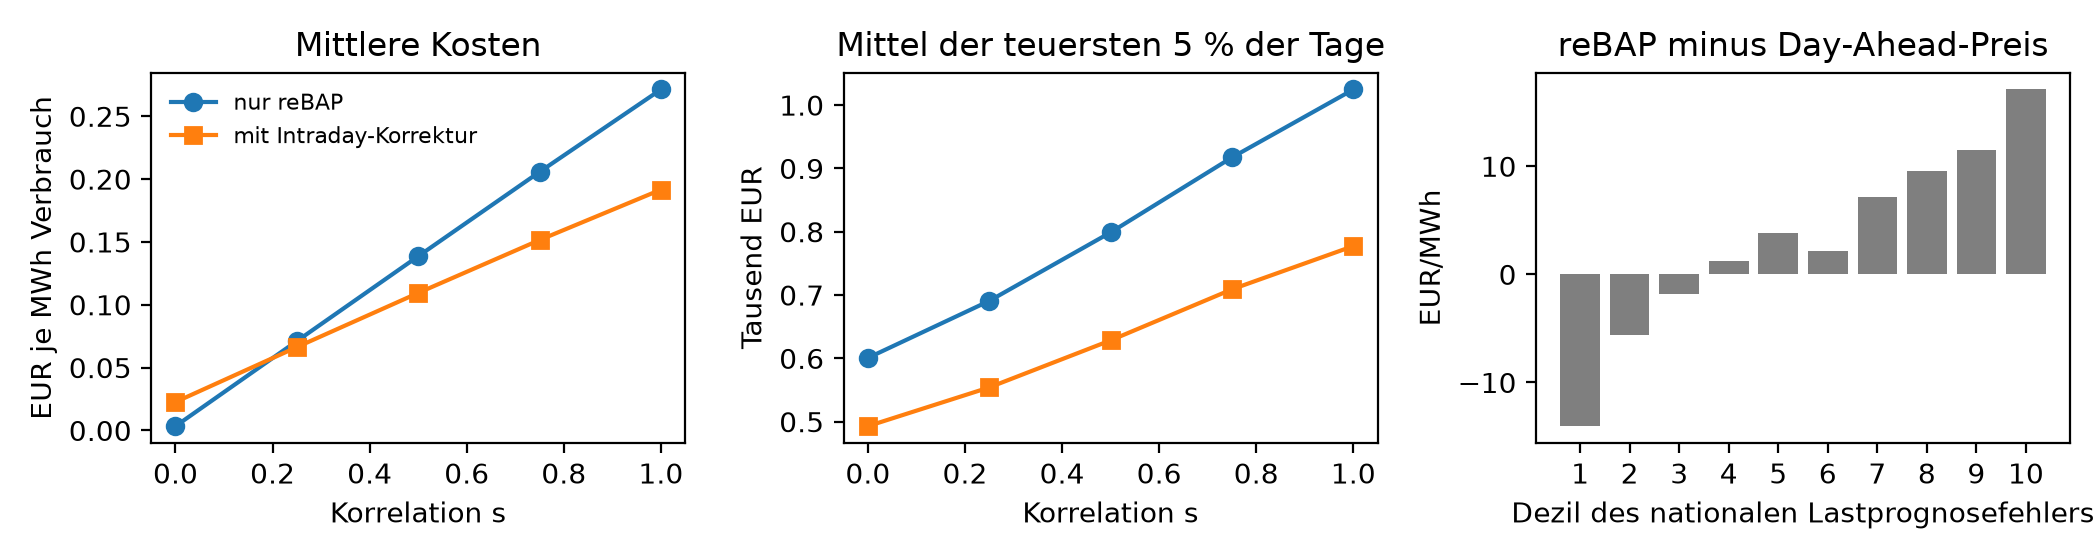
\includegraphics[width=\textwidth]{../figures/balancing_de.png}

\begin{itemize}
\item \textbf{Ein unabhängiger Fehler kostet im Mittel fast nichts, ein mit dem System gleichlaufender Fehler schon.}
Der Abstand zwischen reBAP und Day-Ahead-Preis steigt von $-$14 EUR/MWh im untersten Dezil des nationalen
Lastprognosefehlers auf $+$17 EUR/MWh im obersten. Bei $s = 1$ sind das 0,27 EUR/MWh (rund 27 TEUR je Jahr), mehr
als in jedem von 84 Placebo-Läufen mit um ganze Wochen verschobener Fehlerreihe.
\item Das Risiko bleibt auch bei mittleren Kosten von null und ist konzentriert: Bei $s = 1$ tragen die zehn teuersten
von 638 Tagen 44\,\% der Gesamtkosten.
\item Die Intraday-Korrektur halbiert die offene Energie (von 2,4 auf 1,1\,\% bei $s = 0{,}5$) und senkt die Kosten
der teuersten 5\,\% der Tage um etwa ein Fünftel. Bei $s = 0{,}5$ verschwindet der Vorteil bei den mittleren Kosten
ab etwa 2,4 EUR/MWh halbem Spread. Selbst eine vorab exakt bekannte und zum ID-AEP geschlossene Abweichung kostet bei
$s = 1$ noch 0,14 EUR/MWh: Der Intraday-Preis enthält den gemeinsamen Fehler bereits teilweise.
\end{itemize}

\section{Folgerungen für das Portfoliomanagement}
\begin{itemize}
\item Prognosen nicht nur am mittleren Fehler messen, sondern auch an ihrem Gleichlauf mit dem Systemfehler und an den
Kosten zum reBAP.
\item Intraday dort nachbewirtschaften, wo Messdaten aktuell vorliegen und der Spread klein ist; bei großem Spread
dient die Nachbewirtschaftung vor allem der Risikominderung.
\item Die Pflicht zum Bilanzkreisausgleich (u.\,a. BNetzA-Festlegung BK6-19-212) schließt bewusst offene Positionen
gegen den reBAP aus; die Studie misst allein die Kosten unvermeidbarer Fehler.
\end{itemize}

\section{Erzeugungsseite}
\begin{itemize}
\item Gaskraftwerk mit 400 MW als Tolling, bewertet für 2026: stündlicher innerer Wert 37,1 Mio. EUR, Wert als Reihe
täglicher Spread-Optionen 51,4 Mio. EUR (obere Grenze ohne Anfahrkosten und Rampen).
\item Prognosefehler von Wind und Solar zum reBAP: Eine eigene Prognose aus ICON und ECMWF war ungenauer als die der
Übertragungsnetzbetreiber, kostete aber 1,46 statt 1,74 EUR/MWh (t etwa 2), siehe
\href{https://github.com/serikov-power-markets/de-weather-to-power}{de-weather-to-power}.
\item Investition und Einsatz eines Beispiel-Wärmenetzes mit KWK, Wärmepumpen und Speichern, siehe
\href{https://github.com/serikov-energy-systems/de-district-heating}{de-district-heating}.
\end{itemize}

\section{Grenzen}
Modellierte Terminpreise ohne Risikoprämie; synthetische Prognosefehler ohne Kunden- oder Lieferantendaten; als
Systembezug nur der Lastprognosefehler; ID-AEP ist ein Index und kein handelbarer Kurs; keine Gebühren, Sicherheiten
oder Vertragsstrafen. Forschungsstudie auf öffentlichen Daten.
\end{document}
